\scalebox{0.5}{
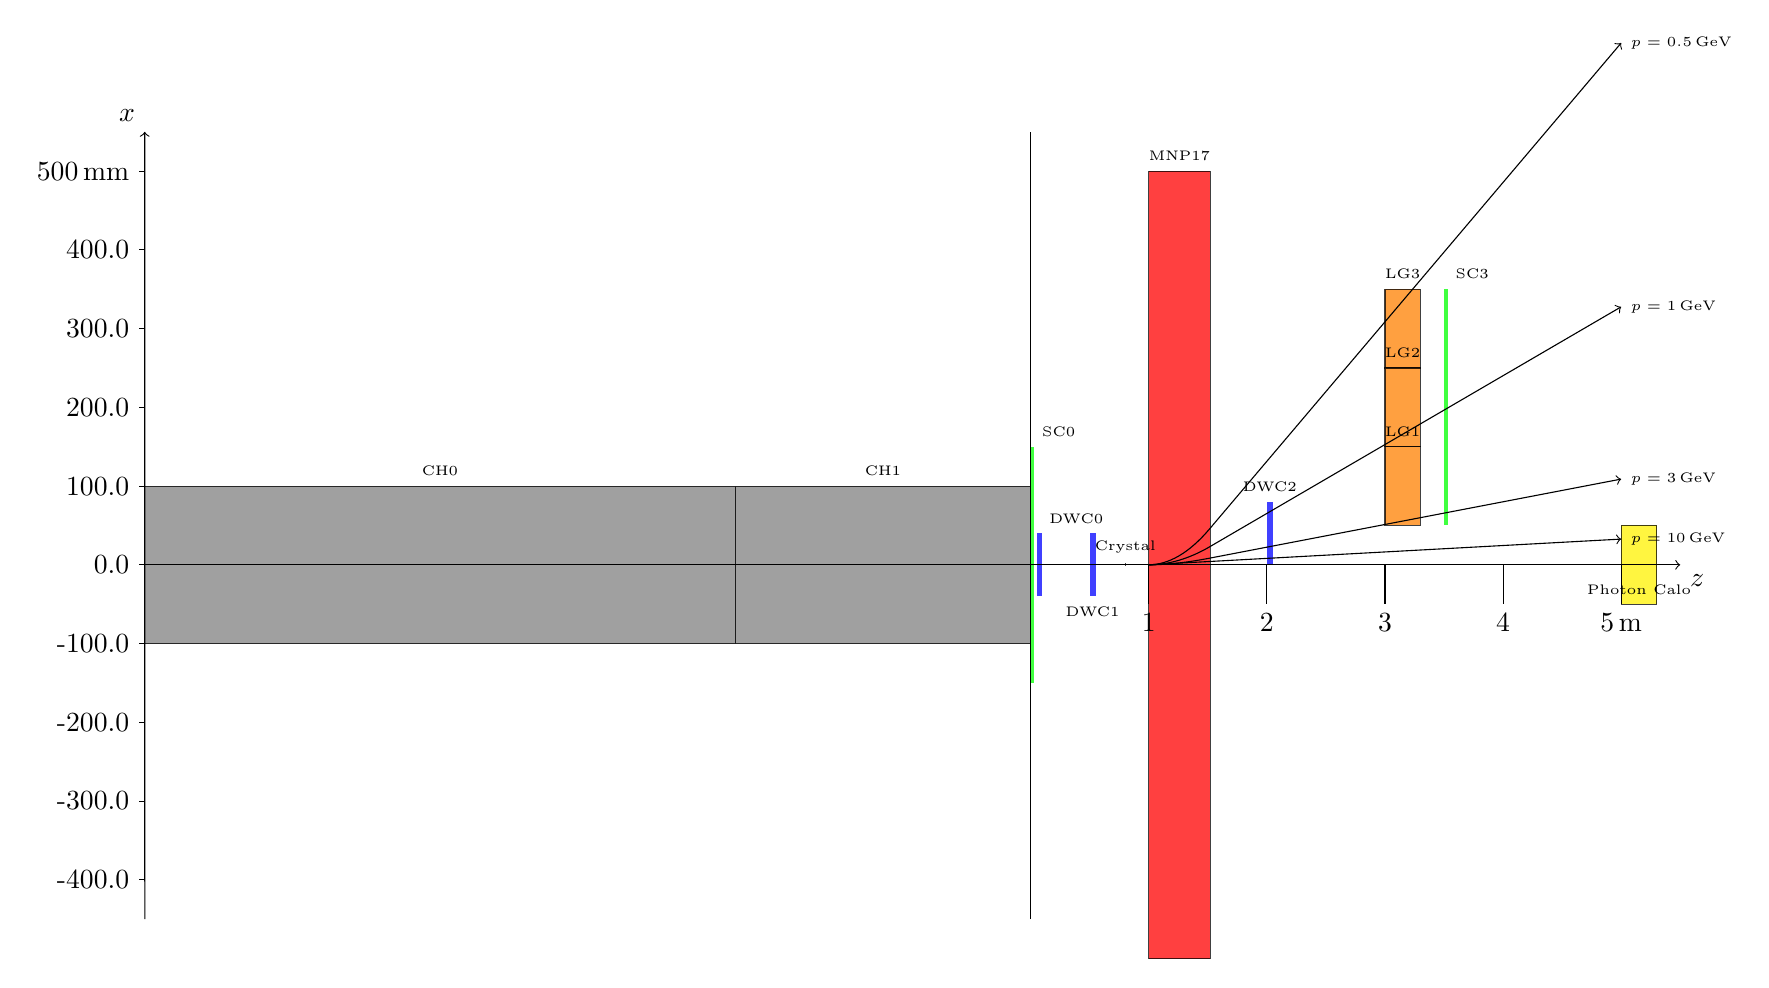
\begin{tikzpicture}[xscale=1.5,yscale=10]

\tikzset{add reference/.style={insert path={%
    coordinate [pos=0,xshift=-0.5\pgflinewidth,yshift=-0.5\pgflinewidth] (#1 south west)
    coordinate [pos=1,xshift=0.5\pgflinewidth,yshift=0.5\pgflinewidth]   (#1 north east)
    coordinate [pos=.5] (#1 center)
    (#1 south west |- #1 north east)     coordinate (#1 north west)
    (#1 center     |- #1 north east)     coordinate (#1 north)
    (#1 center     |- #1 south west)     coordinate (#1 south)
    (#1 south west -| #1 north east)     coordinate (#1 south east)
    (#1 center     -| #1 south west)     coordinate (#1 west)
    (#1 center     -| #1 north east)     coordinate (#1 east)
}}}

\coordinate (ref) at (0,0);
\coordinate (backref) at (-7.5,0);

%% Magnet
\fill[draw=black,fill=red,opacity=0.75,label=north:MNP18] (1,-0.5) rectangle ++(0.52, 1) [add reference=mnp17];
\node[anchor=south] at (mnp17 north) {\tiny{MNP17}};

%% Cherenkov
\fill[draw=black,fill=gray,opacity=0.75] (-2.5,-0.1) rectangle ++(-5, 0.2) [add reference=ch0];
\node[anchor=south] at (ch0 north) {\tiny{CH0}};

\fill[draw=black,fill=gray,opacity=0.75] (0,-0.1) rectangle ++(-2.5, 0.2) [add reference=ch1];
\node[anchor=south] at (ch1 north) {\tiny{CH1}};

%% Scint
\fill[color=green,opacity=0.75] (0,-0.15) rectangle ++(0.03, 0.3) [add reference=sc0];
\node[anchor=south west] at (sc0 north) {\tiny{SC0}};

\fill[color=green,opacity=0.75] (3.5,0.05) rectangle ++(0.03, 0.3) [add reference=sc3];
\node[anchor=south west] at (sc3 north) {\tiny{SC3}};

%% DWC
\fill[color=blue,opacity=0.75] (0.05,-0.04) rectangle ++(0.05, 0.08) [add reference=dwc0];
\node[anchor=south west] at (dwc0 north) {\tiny{DWC0}};

\fill[color=blue,opacity=0.75] (0.5,-0.04) rectangle ++(0.05, 0.08) [add reference=dwc1];
\node[anchor=north] at (dwc1 south) {\tiny{DWC1}};

\fill[color=blue,opacity=0.75] (2,0) rectangle ++(0.05, 0.08) [add reference=dwc2];
\node[anchor=south] at (dwc2 north) {\tiny{DWC2}};

%% Calo
\fill[draw=black,fill=yellow,opacity=0.75] (5,-0.05) rectangle ++(0.3, 0.1) [add reference=photon_calo];
\node[anchor=south] at (photon_calo south) {\tiny{Photon Calo}};

\fill[draw=black,fill=orange,opacity=0.75] (3,0.25) rectangle ++(0.3, 0.1) [add reference=lg3];
\node[anchor=south] at (lg3 north) {\tiny{LG3}};

\fill[draw=black,fill=orange,opacity=0.75] (3,0.15) rectangle ++(0.3, 0.1) [add reference=lg2];
\node[anchor=south] at (lg2 north) {\tiny{LG2}};

\fill[draw=black,fill=orange,opacity=0.75] (3,0.05) rectangle ++(0.3, 0.1) [add reference=lg1];
\node[anchor=south] at (lg1 north) {\tiny{LG1}};

%% Crystal
\fill[color=black,opacity=0.75] (0.8,-0.002) rectangle ++(0.001, 0.004) [add reference=crystal];
\node[anchor=south] at (crystal north) {\tiny{Crystal}};

%% Reference trajectories
\draw[->] (mnp17 west) -- (5,0.0327) node[anchor=west] {\tiny{$p = 10\,\mathrm{GeV}$}};
% \draw[->] (mnp17 west) -- (152,0.27) -- (500,3.27) node[anchor=west] {\tiny{$p = 10\,\mathrm{GeV}$}};
\draw[->] (mnp17 west) arc (-90:-88.3335:17.8695) -- (5,0.1089) node[anchor=west] {\tiny{$p = 3\,\mathrm{GeV}$}};
\draw[->] (mnp17 west) arc (-90:-84.992:5.9565) -- (5,0.3277) node[anchor=west] {\tiny{$p = 1\,\mathrm{GeV}$}};
% \draw[->] (mnp17 west)  arc  (-90:-91:595.7) node[anchor=west] {\tiny{$p = e\,\mathrm{GeV}$}};
\draw[->] (mnp17 west)  arc  (-90:-80:2.978) -- (5,0.6628) node[anchor=west] {\tiny{$p = 0.5\,\mathrm{GeV}$}};

% Draw main coordinate system
\draw[->] (ref) -- ++(5.5,0) node[anchor=north west]{$z$};
\draw (0,-0.45) -- (ref) -- ++(0,0.55);
\draw (backref) -- (ref);
\draw[->] (-7.5,-0.45) -- (backref) -- ++(0,0.55) node[anchor=south east]{$x$};

\foreach \x in {-4,-3,...,4}{
    \pgfmathsetmacro\result{\x * 100}
    \draw (-7.5,0.1 * \x) -- ++(-0.05,0) node[anchor=east]{\result};
}
\draw (-7.5,0.5) -- ++(-0.05,0) node[anchor=east]{500\,mm};

\foreach \z in {1,2,...,4}{
    \draw (\z,0) -- ++(0,-0.05) node[anchor=north]{\z};
}
\draw (5,0) -- ++(0,-0.05) node[anchor=north]{5\,m};

\end{tikzpicture}
}
